\documentclass[12pt, a4paper]{article}
    \usepackage[utf8]{inputenc}
    \usepackage{amsmath, amssymb}
    \usepackage{amsthm}
    \usepackage[dvipsnames,svgnames]{xcolor}
    \usepackage{tikz}
    \usetikzlibrary{arrows.meta, angles, quotes, calc}
    \usepackage[most]{tcolorbox}
    \usepackage[a4paper, total={6.5in, 9in}]{geometry}
    \usepackage{tikz}
    \usepackage{url}
    \usepackage{hyperref}
    \newcommand{\rn}[2]{\tikz[remember picture,baseline=(#1.base)]\node[inner sep=0] (#1) {$#2$};}
    \usetikzlibrary{matrix,arrows.meta}
    \tcbuselibrary{theorems}

    \newtcbtheorem[
    auto counter, 
    number within=section
    ]{theorem}{Theorem}{
    breakable, % <--- Allow page breaks
    colback=RawSienna!10!white, colframe=RawSienna!100!black,
    fonttitle=\bfseries, coltitle=white,
    boxrule=1pt, arc=3pt, left=1mm, right=1mm, top=1mm, bottom=1mm,
    separator sign={.}
    }{thm}

\newtcbtheorem[
    use counter from=theorem
    ]{corollary}{Corollary}{
    breakable, % <--- Allow page breaks
    colback=Orange!10!white, colframe=Orange!100!black,
    fonttitle=\bfseries, coltitle=white,
    boxrule=1pt, arc=3pt, left=1mm, right=1mm, top=1mm, bottom=1mm,
    separator sign={.}
    }{cor}

\newtcbtheorem[
    use counter from=theorem
    ]{remark}{Remark}{
    breakable, % <--- Allow page breaks
    colback=ForestGreen!10!white, colframe=ForestGreen!100!black,
    fonttitle=\bfseries, coltitle=white,
    boxrule=1pt, arc=3pt, left=1mm, right=1mm, top=1mm, bottom=1mm,
    separator sign={.}
    }{rem}
    
\newtcbtheorem[
    use counter from=theorem
    ]{lemma}{Lemma}{
    breakable, % <--- Allow page breaks
    colback=TealBlue!10!white, colframe=TealBlue!100!black,
    fonttitle=\bfseries, coltitle=white,
    boxrule=1pt, arc=3pt, left=1mm, right=1mm, top=1mm, bottom=1mm,
    separator sign={.}
    }{lem}

\newtcbtheorem[
    use counter from=theorem
    ]{definition}{Definition}{
    breakable, % <--- Allow page breaks
    colback=RoyalBlue!10!white, colframe=RoyalBlue!100!black,
    fonttitle=\bfseries, coltitle=white,
    boxrule=1pt, arc=3pt, left=1mm, right=1mm, top=1mm, bottom=1mm,
    separator sign={.}
    }{def}

\newtcbtheorem[
    use counter from=theorem
    ]{example}{Example}{
    breakable, % <--- Allow page breaks
    colback=Blue!10!white, colframe=Blue!100!black,
    fonttitle=\bfseries, coltitle=white,
    boxrule=1pt, arc=3pt, left=1mm, right=1mm, top=1mm, bottom=1mm,
    separator sign={.}
    }{ex}


    \DeclareMathOperator*{\id}{id}
    \DeclareMathOperator{\dist}{d}
    \DeclareMathOperator{\proj}{proj}
    \newcommand{\R}{\mathbb{R}}
    \newcommand{\innp}[1]{\langle #1 \rangle}


    \renewcommand\qedsymbol{$\blacksquare$}
    \renewcommand{\restriction}{\mathord{\upharpoonright}}

    \binoppenalty=\maxdimen
    \relpenalty=\maxdimen

    \title{\textbf{Cops and Robbers: A Graph Theory Game (tentative)}}
\author{Bassel Shoeib \\ ID: 900231376 \\ Mahmoud AlEskandrani \\ ID:900241828 \\ Michael R. Guirgis \\ ID: 900242473 \\ Mohamed A. AboElFotouh \\ ID:900248219 \\ The American University in Cairo}
\date{Spring 2026}


    \begin{document}

    \maketitle

    \vspace{1cm}
\begin{center}
\textit{"Mathematics is the queen of the sciences and number theory is the queen of mathematics."}\\
--- Carl Friedrich Gauss
\end{center}

\vspace{2cm}

\begin{abstract}
    In this paper, we explore the famous graph theory game: Cops and Robbers. We first introduce fundamental concepts related to the game, formally defining cop-winning and robber-winning graphs. We then investigate the game's dynamics on famous graph families, proving lemmas that establish complete graphs and trees as cop-winning, and cycles as robber-winning. Next, we move on to define pitfalls, utilizing this concept to prove a general characterization theorem for cop-winning graphs. Following this, we define the cop number of a graph to analyze multiple-cop winning graphs. Finally, we explore variations of the game, including the lazy cop and cops and attacking robbers.
\end{abstract}

\newpage
%_________________________________________________________________________________________________ Michael _________________________________________________________________________________________________
\section{Introduction}
\textbf{Motivation: }
\begin{definition}{}{}
\textcolor{red}{\textbf{Here we define ``a cop'' and ``a robber'', then we define ``a cop-win graph'' and ``a robber-win graph}}
\end{definition}

\begin{example}{}{}
\textcolor{red}{\textbf{Investigate famous graphs(cycles, trees, complete graphs)}}
\end{example}

%_________________________________________________________________________________________________  Bassel   ______________________________________________________________
\begin{lemma}{}{}
All trees and complete graphs are cop-win graphs. 
\end{lemma}

\begin{lemma}{}{}
All cycles are robber-win graphs.
\end{lemma}
%____________________________________________________________________________________________________
\newpage

\section{Cop-win graphs}

\begin{definition}{Pitfall}{}
Let $G = (V, E)$ be a simple finite graph. 
\begin{itemize}
    \item The \textbf{open neighborhood} of a vertex $x \in V$ is the set of all vertices adjacent to $x$, denoted by $N(x) = \{y \in V : xy \in E\}$.
    \item The \textbf{closed neighborhood} of $x$ is the union of its open neighborhood and the vertex itself, denoted by $N[x] = N(x) \cup \{x\}$.
\end{itemize}
A vertex $u \in V$ is called a \textbf{pitfall} (or a corner) if there exists a distinct vertex $v \in N(u)$ such that its closed neighborhood is a subset of the closed neighborhood of $v$, i.e., $N[u] \subseteq N[v]$. In this case, we say that $v$ \textbf{dominates} $u$.
\end{definition}

\begin{example}{Visualizing a Pitfall}{}
\begin{minipage}{0.65\textwidth}
Consider the graph $G$ shown to the right. Vertex $u$ is a pitfall because its only neighbors are $v$ and $w$. Notice that $N[u] = \{u, v, w\}$ and $N[v] = \{v, u, w, z\}$. Since $N[u] \subseteq N[v]$, $u$ is a pitfall dominated by $v$. If the robber is at $u$, the cop at $v$ can capture the robber in the next move regardless of where the robber flies.
\end{minipage}
\hfill
\begin{minipage}{0.3\textwidth}
\centering
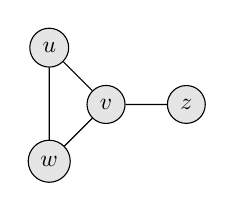
\begin{tikzpicture}[scale=0.85, transform shape, node distance={12mm}, main/.style = {draw, circle, fill=gray!20}] 
\node[main] (1) {$u$}; 
\node[main] (2) [below right of=1] {$v$}; 
\node[main] (3) [below left of=2] {$w$}; 
\node[main] (4) [right of=2] {$z$};
\draw (1) -- (2); \draw (1) -- (3); \draw (2) -- (3); \draw (2) -- (4);
\end{tikzpicture}
\end{minipage}
\end{example}

\begin{theorem}{}{}
A finite graph is cop-win \textit{iff} it can be reduced to a single vertex through the successive removal of pitfalls.
\end{theorem}
\begin{proof}
    We prove this theorem by demonstrating both directions, following the foundational logic established by Nowakowski and Winkler \cite{nowakowski1983vertex}, and independently by Quilliot \cite{quilliot1983jeux}.

    \vspace{0.3cm}
    \noindent\textbf{Forward Direction ($\Rightarrow$): If a graph is cop-win, it is dismantlable.} \\
    Assume $G$ is a finite cop-win graph. We must prove that it contains at least one pitfall, which will allow us to start the dismantling process. Because $G$ is finite and the cop has a winning strategy, any optimally played game must end in a finite number of moves. Let us examine the state of the board exactly \textit{one turn before} the cop wins. 
    
    It is the robber's turn. Let the robber be at vertex $u$ and the cop be at vertex $v$. Because this is the penultimate turn, the cop's strategy guarantees a capture on the very next turn, \textit{no matter what the robber chooses to do}. Consider the robber's options. The robber can either stay at $u$, or move to any adjacent vertex. Therefore, the set of all possible locations where the robber could end their turn is exactly the closed neighborhood of $u$, denoted as $N[u]$.
    
    For the cop (starting at $v$) to guarantee capture on their following turn, they must be able to reach the robber in a single move. This means $v$ must be adjacent to every single vertex the robber could possibly occupy. Mathematically, this requires that every vertex in $N[u]$ is also contained in the closed neighborhood of $v$, meaning $N[u] \subseteq N[v]$. By definition, if $N[u] \subseteq N[v]$, then $u$ is a pitfall dominated by $v$. Thus, any finite cop-win graph must possess at least one pitfall. 
    
    Finally, consider the subgraph $G' = G - \{u\}$. We must ensure that removing $u$ preserves the cop-win property. While removing $u$ strictly reduces the robber's escape paths, one might worry it also breaks the cop's winning strategy if the cop needed to traverse $u$. However, because $N[u] \subseteq N[v]$, any movement the cop originally planned through $u$ can simply be rerouted through $v$ without losing any adjacency or reach. Therefore, the cop's winning strategy on $G$ is perfectly preserved on $G'$, making $G'$ cop-win as well. By repeatedly applying this logic, we can dismantle the graph vertex by vertex until only a single point remains.
    
    \begin{center}
    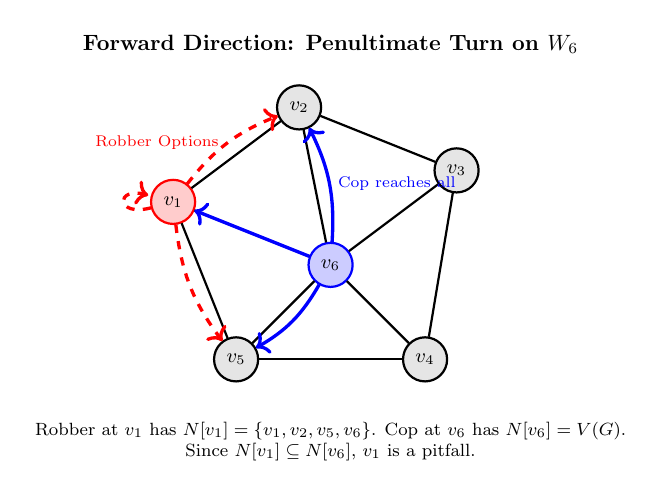
\begin{tikzpicture}[scale=0.8, transform shape, thick, main/.style = {draw, circle, fill=gray!20, minimum size=7mm, font=\small}, 
                        pit/.style = {draw=red, circle, fill=red!20, minimum size=7mm, font=\small}, 
                        dom/.style = {draw=blue, circle, fill=blue!20, minimum size=7mm, font=\small}]
        
        \node[font=\bfseries] at (3.5, 3.5) {Forward Direction: Penultimate Turn on $W_6$};
        
        \node[pit] (u) at (1, 1) {$v_1$}; 
        \node[dom] (v) at (3.5, 0) {$v_6$}; 
        \node[main] (v2) at (3, 2.5) {$v_2$}; 
        \node[main] (v3) at (5.5, 1.5) {$v_3$};
        \node[main] (v4) at (5, -1.5) {$v_4$};
        \node[main] (v5) at (2, -1.5) {$v_5$};
        
        \draw (v) -- (u); \draw (v) -- (v2); \draw (v) -- (v3); \draw (v) -- (v4); \draw (v) -- (v5);
        \draw (u) -- (v2); \draw (v2) -- (v3); \draw (v3) -- (v4); \draw (v4) -- (v5); \draw (v5) -- (u);
        
        \draw[->, dashed, red, very thick] (u) to[bend left=15] node[midway, left, font=\scriptsize] {Robber Options} (v2);
        \draw[->, dashed, red, very thick] (u) to[bend right=15] (v5);
        \draw[->, dashed, red, very thick] (u) edge [loop left] (u);

        \draw[->, blue, very thick] (v) to[bend right=15] node[midway, right, font=\scriptsize] {Cop reaches all} (v2);
        \draw[->, blue, very thick] (v) to[bend left=15] (v5);
        \draw[->, blue, very thick] (v) -- (u);
        
        \node[align=center, font=\footnotesize] at (3.5, -2.8) {Robber at $v_1$ has $N[v_1] = \{v_1, v_2, v_5, v_6\}$. Cop at $v_6$ has $N[v_6] = V(G)$.\\ Since $N[v_1] \subseteq N[v_6]$, $v_1$ is a pitfall.};
    \end{tikzpicture}
    \end{center}

    \begin{center}
    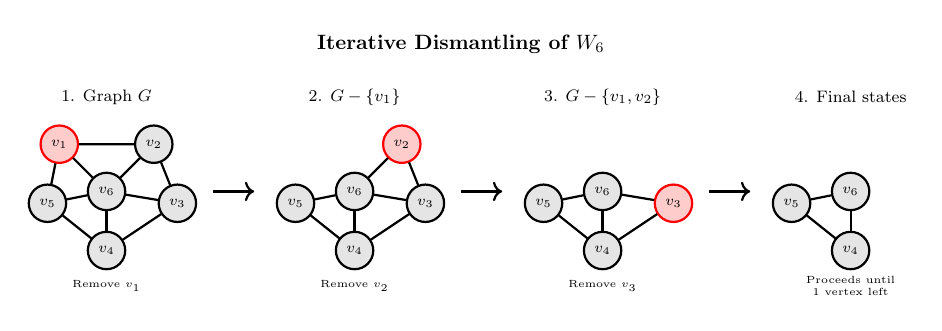
\begin{tikzpicture}[scale=0.75, transform shape, thick, main/.style = {draw, circle, fill=gray!20, minimum size=5mm, font=\scriptsize}, 
                        pit/.style = {draw=red, circle, fill=red!20, minimum size=5mm, font=\scriptsize}]
        
        \node[font=\bfseries] at (6, 2.5) {Iterative Dismantling of $W_6$};
        
        % Step 1
        \begin{scope}[xshift=0cm]
            \node[font=\footnotesize] at (0, 1.6) {1. Graph $G$};
            \node[main] (c) at (0, 0) {$v_6$};
            \node[pit] (1) at (-0.8, 0.8) {$v_1$}; \node[main] (2) at (0.8, 0.8) {$v_2$};
            \node[main] (3) at (1.2, -0.2) {$v_3$}; \node[main] (4) at (0, -1) {$v_4$}; \node[main] (5) at (-1, -0.2) {$v_5$};
            \foreach \x in {1,2,3,4,5} \draw (c) -- (\x);
            \draw (1)--(2)--(3)--(4)--(5)--(1);
            \node[font=\tiny] at (0, -1.6) {Remove $v_1$};
        \end{scope}

        \draw[->, thick] (1.8, 0) -- (2.5, 0);

        % Step 2
        \begin{scope}[xshift=4.2cm]
            \node[font=\footnotesize] at (0, 1.6) {2. $G - \{v_1\}$};
            \node[main] (c) at (0, 0) {$v_6$};
            \node[pit] (2) at (0.8, 0.8) {$v_2$};
            \node[main] (3) at (1.2, -0.2) {$v_3$}; \node[main] (4) at (0, -1) {$v_4$}; \node[main] (5) at (-1, -0.2) {$v_5$};
            \foreach \x in {2,3,4,5} \draw (c) -- (\x);
            \draw (2)--(3)--(4)--(5);
            \node[font=\tiny] at (0, -1.6) {Remove $v_2$};
        \end{scope}

        \draw[->, thick] (6, 0) -- (6.7, 0);

        % Step 3
        \begin{scope}[xshift=8.4cm]
            \node[font=\footnotesize] at (0, 1.6) {3. $G - \{v_1, v_2\}$};
            \node[main] (c) at (0, 0) {$v_6$};
            \node[pit] (3) at (1.2, -0.2) {$v_3$}; \node[main] (4) at (0, -1) {$v_4$}; \node[main] (5) at (-1, -0.2) {$v_5$};
            \foreach \x in {3,4,5} \draw (c) -- (\x);
            \draw (3)--(4)--(5);
            \node[font=\tiny] at (0, -1.6) {Remove $v_3$};
        \end{scope}

        \draw[->, thick] (10.2, 0) -- (10.9, 0);

        % Step 4
        \begin{scope}[xshift=12.6cm]
            \node[font=\footnotesize] at (0, 1.6) {4. Final states};
            \node[main] (c) at (0, 0) {$v_6$};
            \node[main] (4) at (0, -1) {$v_4$}; \node[main] (5) at (-1, -0.2) {$v_5$};
            \draw (c) -- (4); \draw (c) -- (5); \draw (4) -- (5);
            \node[align=center, font=\tiny] at (0, -1.6) {Proceeds until \\ 1 vertex left};
        \end{scope}
    \end{tikzpicture}
    \end{center}

    \vspace{0.3cm}
    \noindent\textbf{Backward Direction ($\Leftarrow$): If a graph is dismantlable, it is cop-win.} \\
    We proceed by induction on the number of vertices, $n = |V(G)|$.
    
    \textit{Base Case:} Let $n = 1$. The graph $G$ consists of a single vertex. The cop places themselves on this vertex and wins immediately. Thus, $G$ is trivially cop-win.
    
    \textit{Inductive Hypothesis:} Assume that any graph with $n$ vertices that can be reduced to a single vertex through the successive removal of pitfalls is cop-win.
    
    \textit{Inductive Step:} Let $G$ be a dismantlable graph with $n+1$ vertices. By definition, $G$ must contain at least one pitfall. Let this pitfall be $u$, and let $v$ be the vertex that dominates it (so $N[u] \subseteq N[v]$). 
    
    Let $G' = G - \{u\}$. Since $G$ is dismantlable, $G'$ is also dismantlable and has $n$ vertices. By our inductive hypothesis, $G'$ is a cop-win graph. We now construct a winning strategy for the cop on the original graph $G$ using a formal retraction (or ``shadow'') strategy. Define a retraction mapping $f: V(G) \to V(G')$ such that $f(x) = x$ for all $x \neq u$, and $f(u) = v$. Because $N[u] \subseteq N[v]$, this mapping ensures that adjacent vertices in $G$ are mapped to adjacent vertices (or the same vertex) in $G'$. When the real robber moves to a vertex $x$ in $G$, the cop imagines a shadow robber moving to $f(x)$ in $G'$. Any legal move by the real robber in $G$ translates to a legal move (or a pass) for the shadow robber in $G'$. 
    
    Since $G'$ is cop-win, the cop executes their optimal strategy on $G$ as if they are chasing the shadow robber on $G'$. In a finite number of steps, the cop will capture the shadow robber at some vertex $c \in V(G')$. This means $c = f(x)$, where $x$ is the current position of the real robber. There are two possibilities at this moment:
    \begin{itemize}
        \item If $c \neq v$, then $f(x) \neq v$, which implies $x = c$. The cop has captured the real robber.
        \item If $c = v$, the shadow robber is caught at $v$, meaning the real robber is either at $v$ (caught) or at $u$. If the real robber is at $u$, it is their turn to move. However, because $N[u] \subseteq N[v]$, any vertex $y$ the robber chooses to move to (or if they stay at $u$) is adjacent to $v$. On the very next turn, the cop simply moves from $v$ to $y$ and captures the robber.
    \end{itemize}
    Thus, $G$ is cop-win.

    \begin{center}
    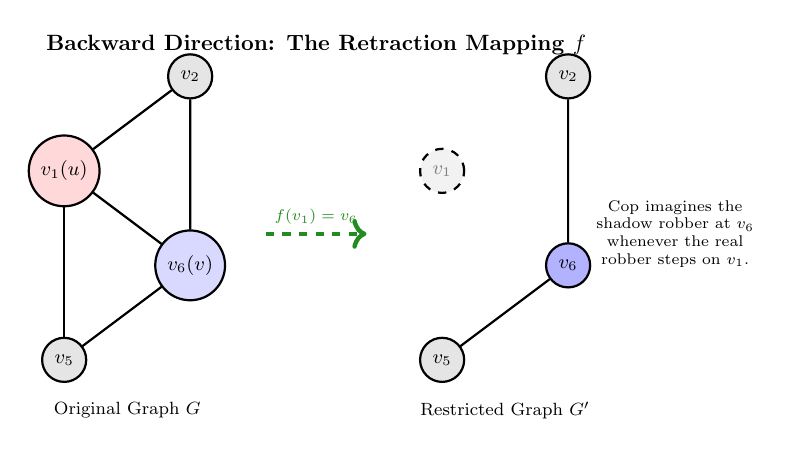
\begin{tikzpicture}[scale=0.8, transform shape, thick, main/.style = {draw, circle, fill=gray!20, minimum size=7mm, font=\small}]
        
        \node[font=\bfseries] at (4, 3) {Backward Direction: The Retraction Mapping $f$};
        
        % Graph G
        \begin{scope}[xshift=0cm]
            \node[main, fill=red!15] (u) at (0, 1) {$v_1 (u)$}; 
            \node[main, fill=blue!15] (v) at (2, -0.5) {$v_6 (v)$}; 
            \node[main] (v2) at (2, 2.5) {$v_2$}; 
            \node[main] (v5) at (0, -2) {$v_5$};
            
            \draw (u) -- (v); \draw (v) -- (v2); \draw (v) -- (v5);
            \draw (u) -- (v2); \draw (u) -- (v5);
            \node[font=\footnotesize] at (1, -2.8) {Original Graph $G$};
        \end{scope}

        \draw[->, ultra thick, ForestGreen, dashed] (3.2, 0) -- (4.8, 0) node[midway, above, font=\scriptsize] {$f(v_1) = v_6$};

        % Graph G'
        \begin{scope}[xshift=6cm]
            \node[main, fill=gray!10, dashed, text=gray] (u) at (0, 1) {$v_1$}; 
            \node[main, fill=blue!30] (v) at (2, -0.5) {$v_6$}; 
            \node[main] (v2) at (2, 2.5) {$v_2$}; 
            \node[main] (v5) at (0, -2) {$v_5$};
            
            \draw (v) -- (v2); \draw (v) -- (v5);
            \node[font=\footnotesize] at (1, -2.8) {Restricted Graph $G'$};
            \node[align=center, font=\scriptsize, text width=3cm] at (3.7, 0) {Cop imagines the\\ shadow robber at $v_6$\\ whenever the real\\ robber steps on $v_1$.};
        \end{scope}
    \end{tikzpicture}
    \end{center}

\end{proof}
\newpage


\section{Multiple Cop graphs}
%_________________________________________________________________________________________________   AboElFotouh, Michael _________________________________________________________________________________________________
Having established the structural characteristics of cop-win and robber-win graphs in the single-cop scenario, we now generalize the analysis to include multiple cops in a graph. Assume, instead of one cop, $k$ cops, denoted by $C_1, \dots, C_k$, are chasing the robber. The cops are placed first on $G$, then the robber. In the cops' turn, only one of them moves.

\begin{definition}{Cop Number}{}
We define the cop number of a graph $G$, $\mathcal{C}(G)$, as the minimum number of cops that is enough to ensure that the cops can catch the robber.
\end{definition}

\begin{remark}{}{}
    Since our analysis involves only simple finite graphs, the cop number is clearly finite since $\mathcal{C}(G) \leq n$ for any graph $G$ where $|G| = n$.
\end{remark}

\begin{definition}{Dominating Set}{}
    A dominating set of a graph $G$ is a set $S \subseteq V_G$ such that every vertex in $G$ is either in $S$ or is adjacent to at least one vertex in $S$.
\end{definition}

\begin{definition}{Domination Number}{}
    The domination number of a graph $G$, $\beta(G)$, is the cardinality of the minimum dominating set of $G$.
\end{definition}

\begin{remark}{}{}
    Given an arbitrary graph $G$, clearly, $\mathcal{C}(G) \leq \beta(G)$.
\end{remark}

\begin{theorem}{}{}
    Any graph $G$ with no 3- or 4-cycles and $\delta(G) \geq n$ has $\mathcal{C}(G) \geq n$.
\end{theorem}
\begin{proof}
    Let $C$ have $n - 1$ cops distributed on the vertices $\{v_1, v_2, \dots, v_{n-1}\}$. Pick a vertex $w$ such that $w \notin \{v_1, \dots, v_{n-1}\}$ (Such $w$ exists as $\delta(G) \geq n, |G| \geq n + 1$). Suppose $w$ has $l$ neighbors and $N(w) = \{v_1, \dots, v_k, w_1, \dots, w_{l-k}\}$ where $w_i \notin \{v_1, \dots, v_{n-1}\}$. Notice that $l \geq n$ and $k \leq n - 1$. Thus, $l - k \geq 1$. For the sake of contradiction, assume $\{v_1, \dots, v_{n - 1}\}$ is a dominating set in $G$. This means that the $N(w_i)$'s must contain one $v_j$. If $j \leq k$, then there exists a 3-cycle $(w, w_i, v_j, w)$, a contradiction. So, we get that $j \geq k + 1$. Also, since $G$ has no 4-cycle, $N(w_i) \cap N(w_m) = \{w\}$ for $i \neq m$. So, every $w_i$ must be adjacent to a unique $v_j$. Counting the total number of vertices in the dominating set, we get that $|\{v_1, \dots, v_{n - 1}\}| \geq k + (l - k) = l$. Thus, $n -1 \geq l$, a contradiction.\\\\
    Hence after placing the cops, say $\{C_1,\dots, C_{n-1}\}$, $R$ is able to place himself on a vertex $r$ which is neither equal to nor adjacent to any of the $C_i$'s. But $R$ can keep up this situation because, after every move of the cops, at most $n-1$ of $R$’s neighbors are covered by cops (no 3- or 4-cycles), thus allowing $R$ to go to the free neighbor. 
\end{proof}
\begin{theorem}{}{}
    Any planar graph $G$ has $\mathcal{C}(G) \leq 3$.
\end{theorem}

\begin{proof}
    
\end{proof}
%_________________________________________________________________________________________________
\newpage
\section{Variations of Cops and robbers}
\subsection{Lazy Cops and Robbers Variation}

\subsection{Attacking Robbers Variation}

\subsection{Drunk Robbers Variation}

\end{document}